\subsection{Android}
	Das Unternehmen Android wurde 2003 von Andy Rubin gegründet und wurde 2005 von Google aufgekauft. Seitdem kümmert sich Google und das Android Open Source Project (AOSP) um die Weiterentwicklung des Systems. Zuletzt wurden die neuen Versionen jeweils von Google intern entwickelt und zum Release der Version der AOSP Community als Open-Source bereitgestellt. Das Betriebssystem wird in den meisten Fällen von den Smartphone Herstellern, oder Entwicklerteams, noch weiter angepasst, bevor es für die einzelnen Geräte bereitgestellt wird.\\
	
	Basis für das Betriebssystem ist ein modifizierter Linux-Kernel und eine Java Virtual Machine (JVM)\cite{ArtDalvik}. Bis einschliesslich Version 4.4 wurde hierfür die Dalivk Runtime und für alle neueren Versionen die Android Runtime (ART) verwendet. Jede App l"auft in einer eigenen Instanz der entsprechenden Runtime und in einer Sandbox.\newline
	Oberhalb der JVM sind die meisten Komponenten in Java implementiert.\\
	
	\begin{figure}[h]
		\centering
		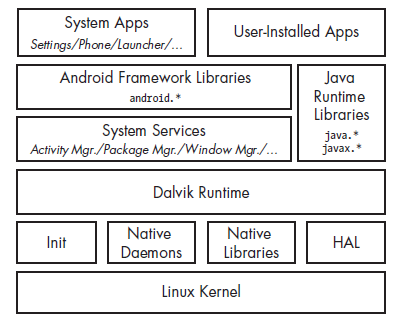
\includegraphics[width=0.7\linewidth]{android_pages/graphics/architektur_android_.png}
		\caption{Die Android Architektur \protect\cite[S. 2]{Elenkov2014} }
		\label{fig:architektur_android}
	\end{figure}
	
\subsubsection{Die Dalvik- und Android Runtime}
	Ein grundsätzlicher Unterschied zwischen einer klassischen JVM, wie sie auf dem Desktop und anderen Geräten zum Einsatz kommt, und einer Runtime die auf Android läuft ist der, dass auf Android die Runtime auf einer Register- anstatt auf einer Stackmaschine basiert\cite{DalvikBytecode}. Somit unterscheidet sich der Bytecode zwischen den Plattformen. Eine Registermaschine bringt mehrere Vorteile mit, unter anderem ist der Bytecode kleiner, was gerade mobilen Endgeräten entgegen kommt.
	Zusätzlich wird nicht mehr mit den üblichen \textit{jar}- und \textit{class}-Dateien, sondern mit einem eigenen Format namens \textit{.dex} gearbeitet\cite{DexFormat}. Dieses ist für den mobilen Einsatz optimiert.\\\\
	Die Dalvik Runtime stammt noch aus dem ursprünglichen Android Projekt, und ähnelt einer klassischen JVM noch sehr. Sie interpretiert Bytecode zur Laufzeit und ist in der Lage oft genutzten Code zur Laufzeit zu kompilieren (\textit{Just-in-time-Compilation, kurz: JIT}). \\
	Die größte Änderung mit dem Umstieg auf die Android Runtime ist, dass nun vorkompilierter Programmcode (\textit{Ahead-Of-Time-Compilation}, kurz: \textit{AOT}) genutzt wird. Der Hintergrundgedanke dieser Veränderung ist, dass dadurch die Performance deutlich verbessert wird. Allerdings ist native kompilierter Code größer als Bytecode, wodurch wiederum mehr Speicher auf den Geräten benötigt wird.
	Da Android auf vielen verschiedenen Hardware Plattformen laufen soll und der native Code Plattform abhängig ist, wird der Bytecode während der Installation in Nativen kompiliert.\\
	Durch das Nutzen von Java, wird Exploits welche auf Basis von Bufferoverflows arbeiten entgegen gewirkt, da Java die Speicherzugriffe überprüft und bei Überläufen eine Exception wirft, was den Abbruch der auslösenden Operation als Folge hat. Dieser Schutz ist allerdings nur unter der Nutzung von Java-Programmcode vorhanden und nicht wenn nativer, z.B. durch den Einsatz des Java-Native-Interfaces (\textit{JNI}), genutzt wird.